% Условная компиляция для самостоятельной работы
\ifdefined\mainfile
    % Если это часть основного файла, не добавляем начало и конец документа
\else
    \documentclass[12pt, a4paper]{report}
    \usepackage{/Users/vladbelousov/Desktop/Semestr_4-FP-NSU/Настройка/library}
    \usepackage[utf8]{inputenc} % Подключение поддержки UTF-8
    \begin{document}
\fi

%%-------------------------------%%

\[ E_x (\vec{r } ,t ) = A \cos (k_x x ) \sin (k_y y ) \sin (k_z z) e^{- i \omega t}  \] 

\[ E_y (\vec{r } ,t ) = B \sin (k_x x ) \cos (k_y y ) \sin (k_z z) e^{- i \omega t} \] 

\[ E_z (\vec{r } ,t ) = D \sin (k_x x ) \sin (k_y y ) \cos (k_z z) e^{- i \omega t} \] 

\[ A k_x  + B k_y + D k_z = 0 \Rightarrow ((\overrightarrow{A,B,D}, (k_x, k_y, k_z)  )) = 0 \] 

\begin{center}
    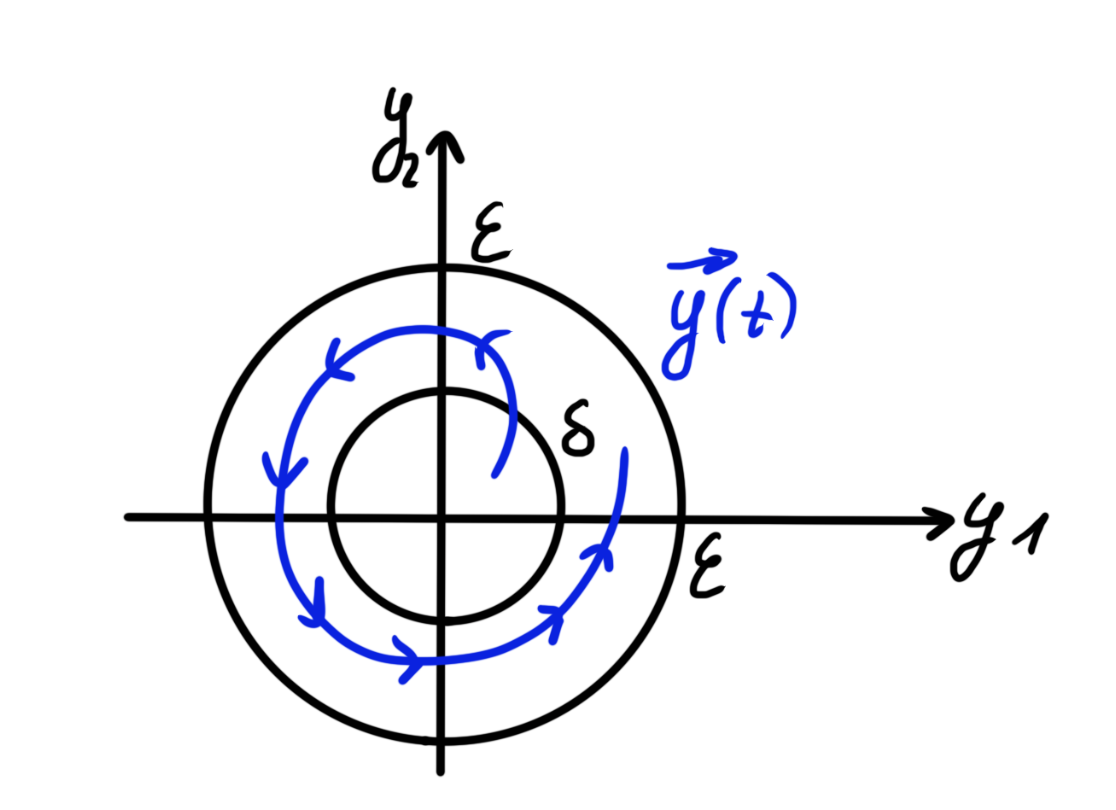
\includegraphics[width=0.3\textwidth]{/Users/vladbelousov/Desktop/Semestr_4-FP-NSU/ЭиО/Лекции_по_дням/image/48.png}
\end{center}

Пример: \( \displaystyle A_1 =1 , \text{ }  B_1= 0 , \text{ }  D_1 = -\frac{k_x}{k_z}  \) 

\[ (\overrightarrow{A_2,B_2, D_2}  ) = \left[ (\overrightarrow{A_1,B_1, D_1}  ) \times \frac{\vec{k} }{|k|} \right]\] 

\( \Rightarrow  \)  для \( \forall  \)  вектора \( \vec{k } (|\vec{k} \neq 0 |)  \exists \) плоскость \( \perp \vec{k}  \), в которой можно выбрать два линейно независимых (ортогональных) вектора \( \overrightarrow{A_1, B_1, D_1}   \)  и \( \overrightarrow{A_2, B_2, D_2} \), которые являются амплитудами собственных колебаний и имеют одну и ту же частоту:

\[ \displaystyle \underbrace{\frac{\omega ^2 \varepsilon \mu }{c ^2 }}_{k ^2} = k_x ^2 + k_y ^2 + k_z ^2 \quad \text{(т.е. двухкратное вырождение).}  \] 

Пример: если a= b, тогда решение с \( n_x, n_y ,n_z \)  имеет ту же частоту, что и решение \( n_y, n_x, n_z \to  \)  четырех кратное вырождение.

Магнитное поле моды \( n_x, n_y, n_z \):

\[ \omega_{ n_x, n_y ,n_z}  = \frac{c}{\sqrt{\varepsilon \mu}} \sqrt{\left( \frac{\pi n_x}{a}  \right) ^2+ \left( \frac{\pi n_y}{b}  \right) ^2+ \left( \frac{\pi n_z}{d}  \right) ^2} , \quad  (\varepsilon = \mathrm{cosnt} , \text{ } \mu = \mathrm{cosnt}  ) \] 

\[ \vec{B } (\vec{r } , t ) = \frac{c}{i \omega_{ n_x, n_y ,n_z}}  \mathrm{rot } \vec{E} (\vec{r}  ,t )  \] 

\section{Связь мод резонатора с плоскими волнами}

\[ E_x(\vec{r } , t ) = -\frac{A}{8}  (e^{i k_x x} +e^{-i k_x x} )(e^{i k_y y} -e^{-i k_y y} )(e^{i k_z z} -e^{-i k_z z} )e^{- i \omega t} =   \] 

\[ = c_1 e^{i k_x x + i k_y y + i k_z z - i \omega t} +c_2 e^{-i k_x x + i k_y y + i k_z z - i \omega t} +... c_8 e^{...}   \] 

- восемь плоских волн.

\begin{center}
    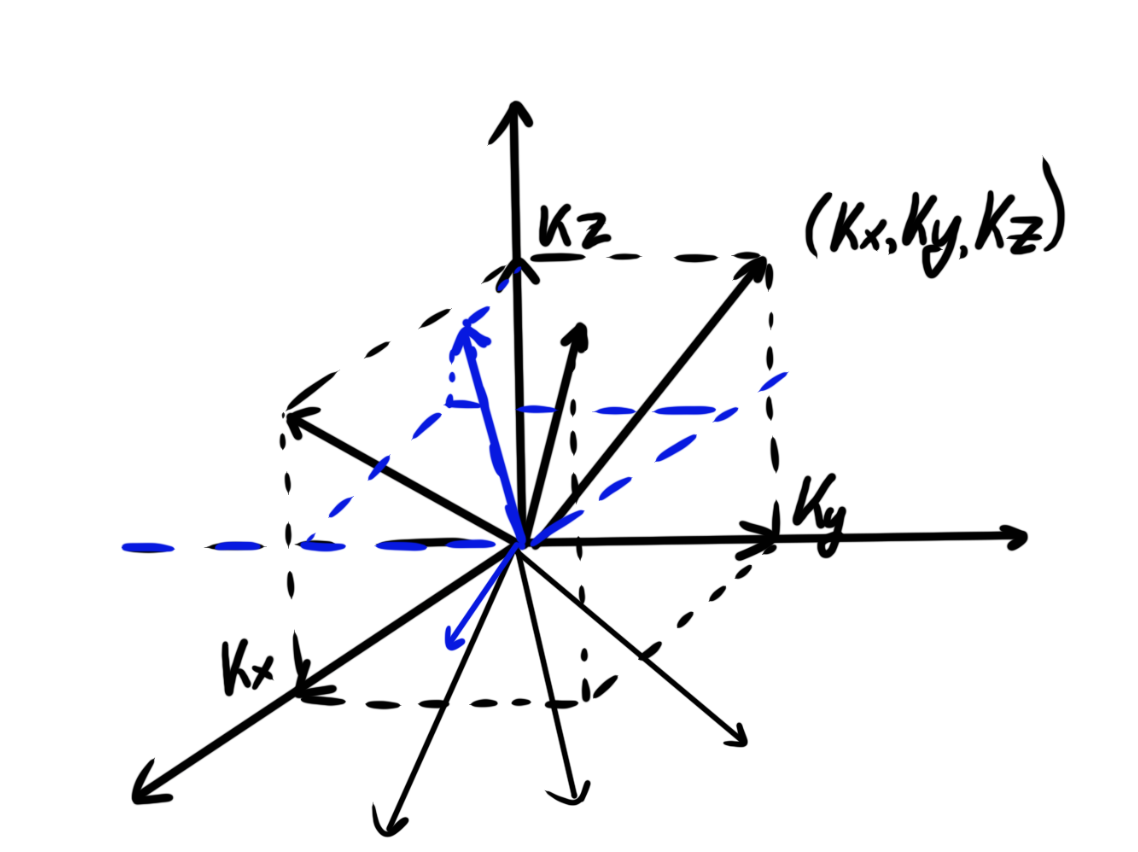
\includegraphics[width=0.5\textwidth]{/Users/vladbelousov/Desktop/Semestr_4-FP-NSU/ЭиО/Лекции_по_дням/image/49.png}
\end{center}

\section{Минимальная частота мод}

\[ \omega_{0,0,0} - \text{ не бывает} ,\quad \omega_{0,0,n_z} - \text{ не бывает } (\text{если два индекса равны 0, то решений нет} )   \] 

\[ \omega_{1,1,0} =\frac{c}{\sqrt{\varepsilon \mu } } \sqrt{\left( \frac{\pi}{a}  \right) ^2 + \left( \frac{\pi}{b}  \right) ^2}  , \quad \omega_{1,0,1} = \frac{c}{\sqrt{\varepsilon \mu } } \sqrt{\left( \frac{\pi}{a}  \right) ^2 + \left( \frac{\pi}{d}  \right) ^2} , \quad \omega_{0,1,1} = \frac{c}{\sqrt{\varepsilon \mu } } \sqrt{\left( \frac{\pi}{b}  \right) ^2 + \left( \frac{\pi}{d}  \right) ^2}  \] 


Если \( a>b>d ,  \) то \( \omega_{1,1,0}  \) - минимальная частота \( \Rightarrow  \) основная мода резонатора\dots

Поле основной моды: 

\[ E_x = E_y = 0  , \quad  \mathrm{Re}  (E_z (\vec{r } , t )) = E_0 \sin (k_x x)\sin  (k_y y)\cos (\omega_{1,1,0} t) \]

\begin{center}
    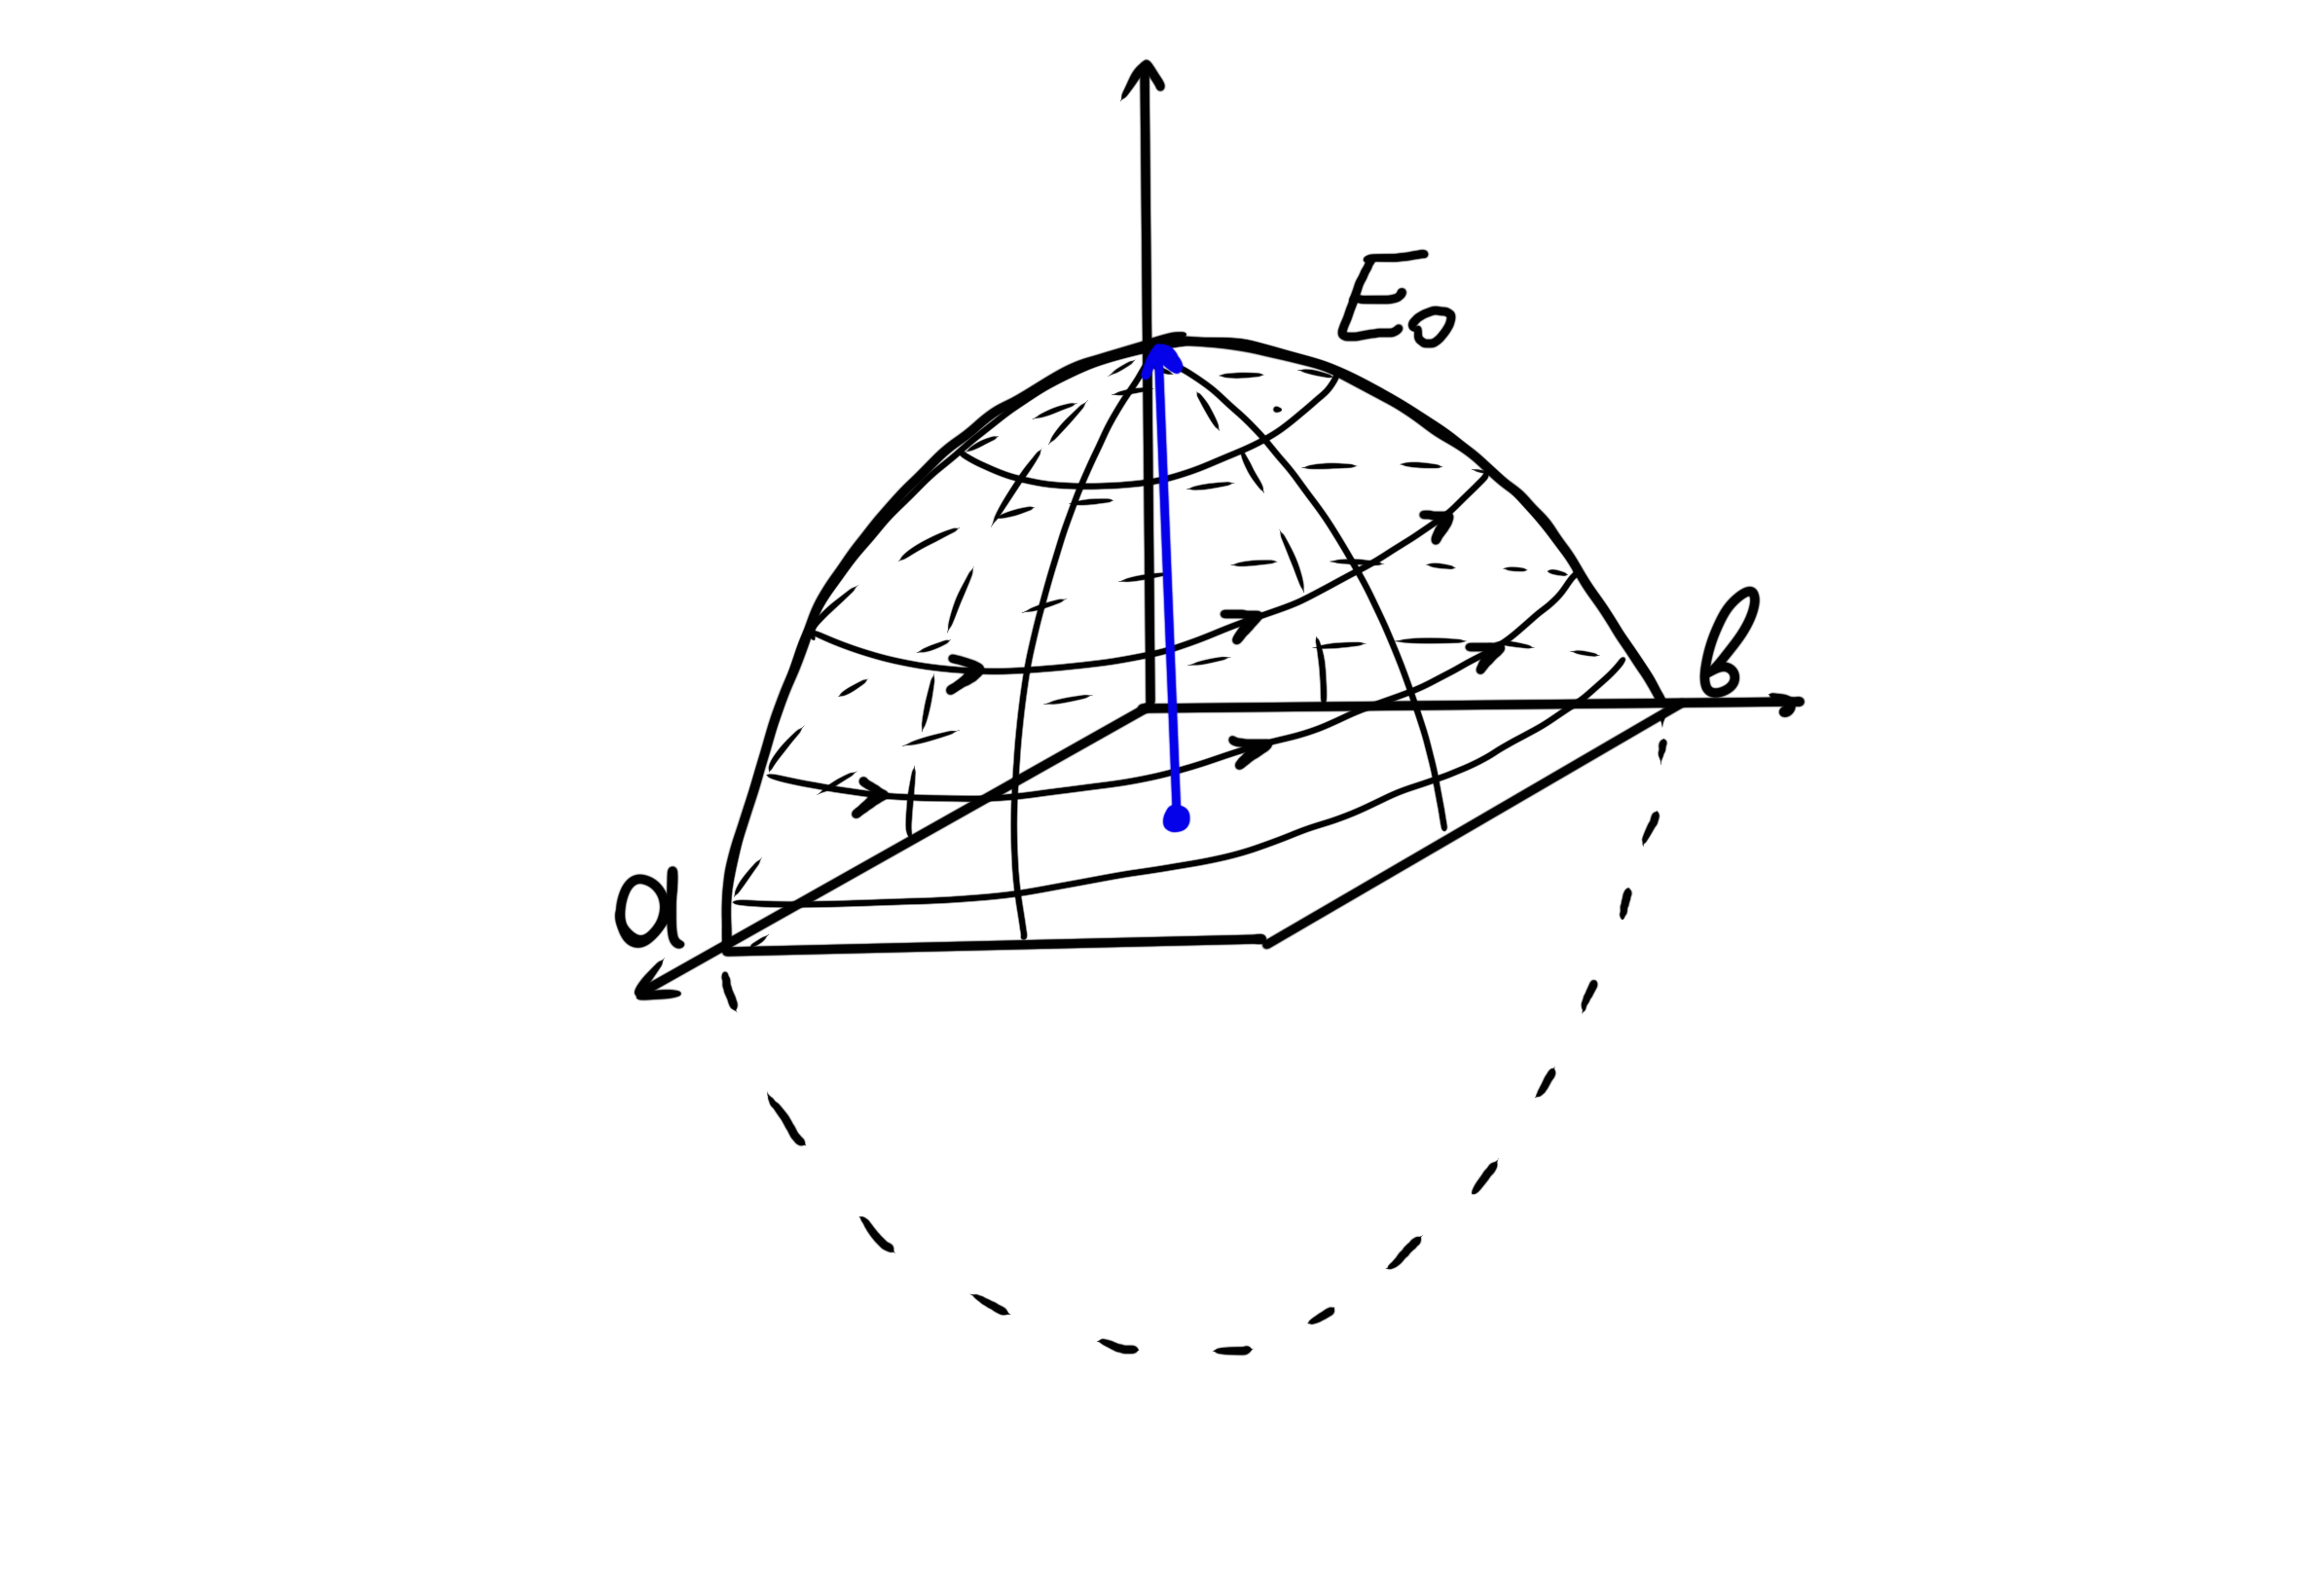
\includegraphics[width=0.5\textwidth]{/Users/vladbelousov/Desktop/Semestr_4-FP-NSU/ЭиО/Лекции_по_дням/image/50.png}
\end{center}

\[ \vec{B }  = - \frac{c}{\omega_{1,1,0} }  \left[ \vec{e_x} k_y \sin (k_x x ) \cos (k_y y ) - \vec{e_y } k_x \cos (k_x x ) \sin (k_y y )   \right]  \sin (\omega_{1,1,0} t)\] 

\section{Влияние конечной проводимости стенок на частоты мода резонатора}

Рассматриваем случай, когда электромагнитные поля мод проникают в стенки резонатора на глубину \(\displaystyle  \delta \sim \frac{c }{\sqrt{2 \pi \mu \sigma \omega}} \ll a, b,d  \). Найдем время затухания моды в резонаторе. 

\[ E,B \sim e ^{-i \omega t } = e^{ - i (\omega ' - i\omega '')t} , \text{ где } \omega' = \mathrm{Re} (\omega) , \text{ } \omega'' =-\mathrm{Im} (\omega)  \quad (\omega =\omega ' - i \omega'')   \] 

Пусть \( \varepsilon = \mathrm{cosnt}, \text{ }  \mu = \mathrm{cosnt}.   \) 

\[ \overline{W}_E - \text{(полная энергия поля в резонаторе, усредненная по t)} = \int dV \frac{\varepsilon (\overline{\mathrm{Re}\vec{E} (\vec{r } ,t ) }  ) ^2 }{8 \pi}  \boxed{=}  \] 

\[(\overline{\mathrm{Re}\vec{E} (\vec{r } ,t ) }  ) ^2 = \left( \overline{\frac{\vec{E }  (\vec{r } ) e^{- i (\omega ' - \omega '')t} + \vec{E } ^{* }  (\vec{r } ) e ^{ i \omega ' t - \omega ' t} }{2} }   \right)  \] 

\[ \boxed{= } \int  \frac{dV \varepsilon}{8 \pi}  \left\{\overline{ \frac{(\vec{E } (\vec{r }) \vec{E } (\vec{r } ) ) e^{- 2 i \omega 't } + (\vec{E } ^{* } (\vec{r } ), \vec{E } ^{* } (\vec{r } )) e ^{ 2 i \omega ' t} + 2 (\vec{E } (\vec{r } ), \vec{E} ^{* } (\vec{r } )) }{4} }   \right\} e^{- 2 \omega ''t }  \] 

\[ \overline{e ^{ -2 i \omega ' t } }  =\overline{\cos (2 \omega ' t)- i \sin (2 \omega ' t)} = 0 \quad (\text{ за период } T =\frac{ 2\pi}{\omega'} )     \] 

\[ \Rightarrow \overline{W_E} = \int dV \frac{\left\lvert \vec{E } (\vec{r } ) \right\rvert ^2 \varepsilon}{1 6\pi } e^{- 2 \omega '' t}     \] 

\[ \overline{W_B} = \int dV \frac{\left\lvert \vec{B } (\vec{r } ) \right\rvert ^2}{1 6\pi }\frac{1}{\mu}  e^{- 2 \omega '' t}    \] 


\begin{center}
    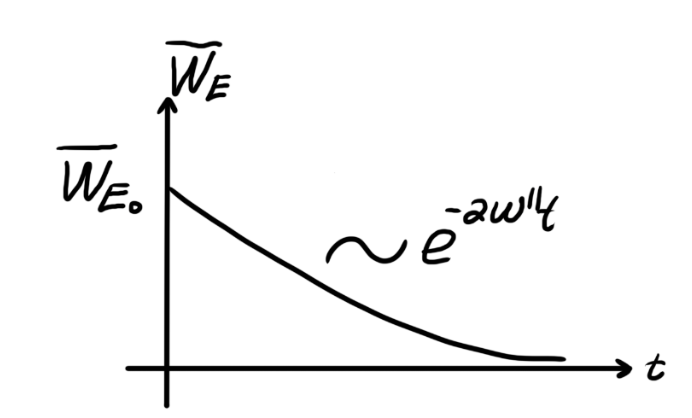
\includegraphics[width=0.4\textwidth]{/Users/vladbelousov/Desktop/Semestr_4-FP-NSU/ЭиО/Лекции_по_дням/image/52.png}
    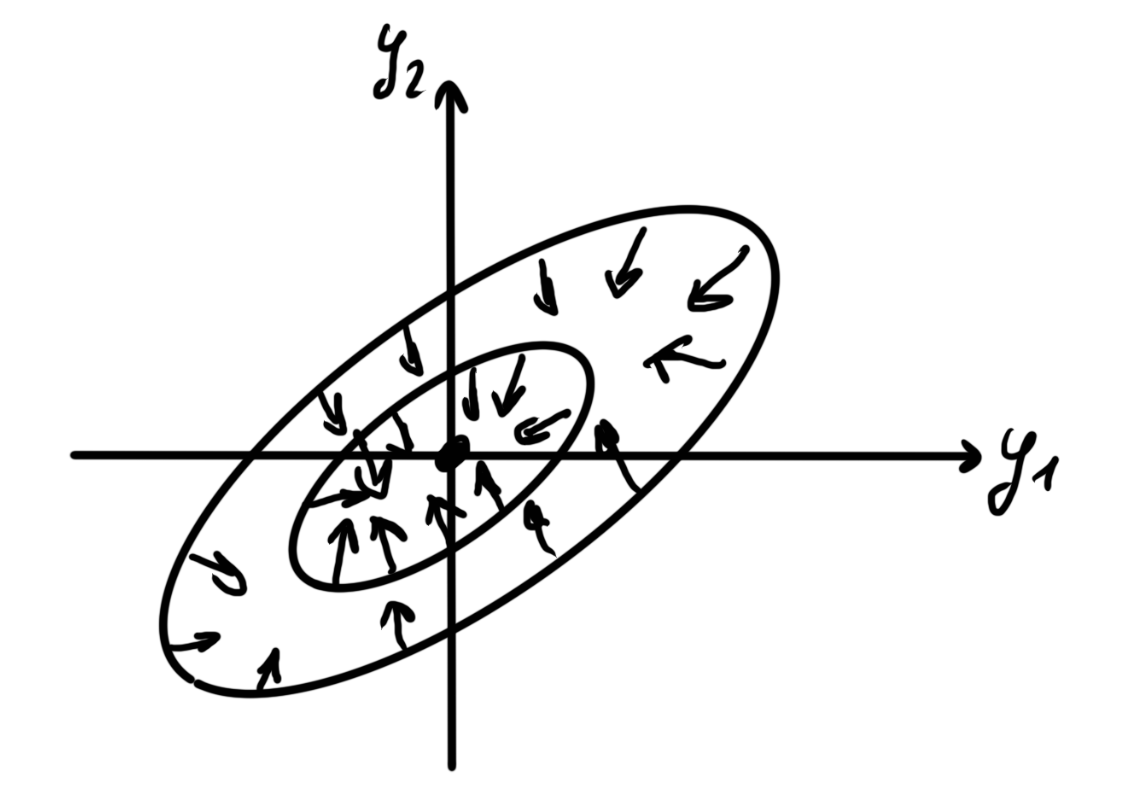
\includegraphics[width=0.3\textwidth]{/Users/vladbelousov/Desktop/Semestr_4-FP-NSU/ЭиО/Лекции_по_дням/image/53.png}
\end{center}

\[ \overline{W }  = \overline{W_E} + \overline{W_B}  = \overline{W_0 } e^{ - 2 \omega '' t}  \quad  \frac{d \overline{ W}  }{dt } = - 2 \omega '' \overline{W }(t)  \] 

Потери энергии в стенках резонатора: \( \displaystyle \oint \left( \overline{\vec{\mathbb{S}} },ds \right)   = \frac{c}{ 16 \pi}  \sqrt{\frac{ \mu \omega '}{2 \pi \sigma} } \oint_{S} \left\lvert \vec{H } _{\tau } (\vec{r})   \right\rvert ^2 ds \,  e^{ - 2 \omega '' t} \) 

\[  \overline{\vec{\mathbb{S}}}   - \text{вектор Пойнтинга} , \quad S - \text{площадь стенок резонатора}   \] 

\[ \omega ''  = \frac{\frac{c}{ 16 \pi } \sqrt{\frac{ \mu \omega' }{2 \pi \sigma} } \displaystyle  \oint _{S} \left\lvert \vec{H } _{\tau } (\vec{r})   \right\rvert ^2 ds \, e^{- 2 \omega '' t}}{ \frac{1}{8 \pi } \displaystyle \int dV \left(  \varepsilon \left\lvert \vec{E } (\vec{r } ) \right\rvert ^2 + \frac{1}{\mu} \left\lvert \vec{B } (\vec{r } ) \right\rvert  ^2 \right)e^{- 2 \omega '' t} }   \] 

\[ Q = \frac{ \omega ' }{2  \omega '' } - \text{добротность}   \] 

Свойства резонатора с \( \omega '' = 0 (Q \to  \infty )  \)  (Ландау, Лифшиц)

\[ \int_{V} \frac{\varepsilon \left\lvert \vec{E } (\vec{r } ) \right\rvert ^2  dV}{16 \pi} = \int_{V} \frac{1}{\mu } \frac{\left\lvert \vec{B } (\vec{r } ) \right\rvert ^2  dV}{16 \pi} ,\quad   \text{ для } \varepsilon = \mathrm{cosnt}(\omega),  \text{ } \mu = \mathrm{cosnt}(\omega)    \] 

\section{Волноводы   }

- труба с идеально проводящими стенками однородная по  сечениям вдоль своей оси. Применение - транспортировка электромагнитных волн (энергии и информации) с малыми потерями на значительные расстоянияы.

\begin{center}
    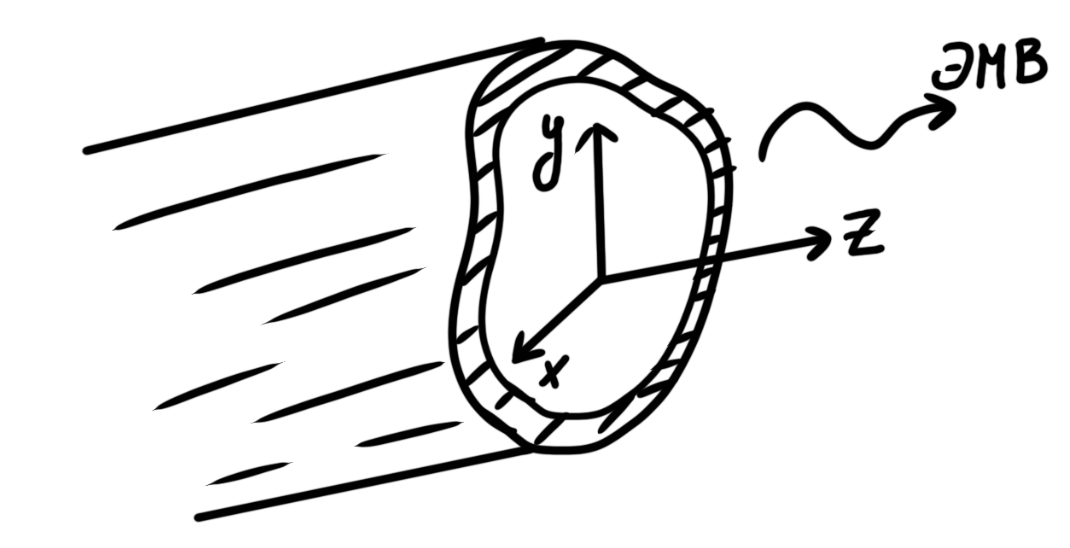
\includegraphics[width=0.5\textwidth]{/Users/vladbelousov/Desktop/Semestr_4-FP-NSU/ЭиО/Лекции_по_дням/image/51.png}
\end{center}

\[ \underset{\text{поле бегущей волны} }{\vec{E } (\vec{r } , t )}  = \vec{E }  ( x, y ) e^{ i k_z z  - i \omega t } , \quad  \vec{B } (\vec{r }, t          )  = \vec{B }  ( x, y ) e^{ i k_z z  - i \omega t }  \] 

\[ \mathrm{rot } (\vec{E } (x,y )e^{i k_z z}) = \frac{i \omega }{c } ( \vec{B } (x,y ) e^{ i k_z z} )     \] 

\[ \mathrm{rot } (\vec{H } (x,y )e^{i k_z z}) = -\frac{i \omega }{c } ( \vec{D} (x,y ) e^{ i k_z z} )  \] 

Выделим поперечные компоненты этих уравнений: 

\[[ \vec{e_{z} } \times [ \nabla \times  \vec{E } (x,y ) e^{i k_z z} ]] = \frac{i \omega }{c } [ \vec{e_z } \times  \vec{B } (x,y) e^{ i k_z z}  ]  , \quad  \begin{aligned}
    \vec{B } (x,y ) = \mu(\omega ) \vec{H}(x,y ) \\ 
    \vec{D} (x,y ) = \varepsilon(\omega ) \vec{E}(x,y )
\end{aligned}    \] 

\[ \nabla (E_z (x,y ) e^{ i k_z z } ) - \frac{\partial}{\partial z} (\vec{E } (x,y )e^{i k_z z} ) = \frac{i \omega }{c } [\vec{e_z} \times \vec{B } (x,y ) e^{ i k_z z} ]\text{  }  (z-\text{ая компонента уравнения } \equiv 0)  \] 

\[ (\nabla_{\perp } E_z (x,y ) ) e^{i k_z z} - \vec{E } _{ \perp } (x,y ) e^{i k_z z} =  \frac{i \omega }{c } \vec{B} _{ \perp } (x,y )    e^{ i k_z z}      \] 

\[ \nabla_{ \perp } H_z (x,y )- H_{ \perp } (x,y ) i k_z = - \frac{ i\omega }{c } \vec{D } _{\perp  } (x,y)  \]  

%%-------------------------------%%

% Закрытие документа, если файл компилируется отдельно
\ifdefined\mainfile
    % Если это основной файл, не нужно заканчивать документ
\else
    \end{document}
\fi